\section{FSM por comportamiento (estilo \textit{One-Hot}) \label{sec:s4}}

\begin{center}
	\begin{minipage}{12cm}
		\begin{tcolorbox}[title=Actividad 4]
			Repetir el inciso 3 pero indicando codificación \textit{``ONE - HOT''}. ¿Qué códigos \textit{ONE-HOT} fueron utilizados, como los de la tabla normal o la modificada?
		\end{tcolorbox}	
	\end{minipage}
\end{center}

La visualización RTL de la FSM, descrita por comportamiento en estilo \textit{One-Hot}, se muestra en la \autoref{fig:FSM_Behavior_OneHot_RTL}. En comparación a la Actividad 1 y 2, se implementan solo 2 compuertas lógicas OR, un multiplexor de 4 bits, un selector, un flip-flop D y dos registros de estados. En la \autoref{fig:FSM_Behavior_OneHot_Graph} se observa el diagrama de estados reportado por el \textit{State Machine Viewer}, que corresponde con el diagrama visto en clase. Además, en la \autoref{fig:FSM_Behavior_OneHot_Table} se tiene la tabla de códigos utilizada por el software de Quartus, que corresponde al estilo \textit{One-Hot} modificado. Finalmente, en la \autoref{fig:FSM_Behavior_OneHot_Tran} se hallan todas las transiciones de los estados y que condición se debe dar para hacer el cambio del estado actual al estado destino.

Las simulaciones se visualizan en la \autoref{fig:FSM_Behavior_OneHot_Wave}. El comportamiento es el mismo que el descrito en actividades anteriores.

En los Anexos se localiza la descripción de la FSM descrita por comportamiento y en estilo \textit{One-Hot}. La única diferencia de este código con el de la Actividad 3, es el tipo de codificación utilizada en parámetros, ya que se utilizó el \textit{One-Hot}, no obstante, Quartus implementará siempre el estilo \textit{One-Hot} modificado.

\begin{figure}[ht]
	\centering
	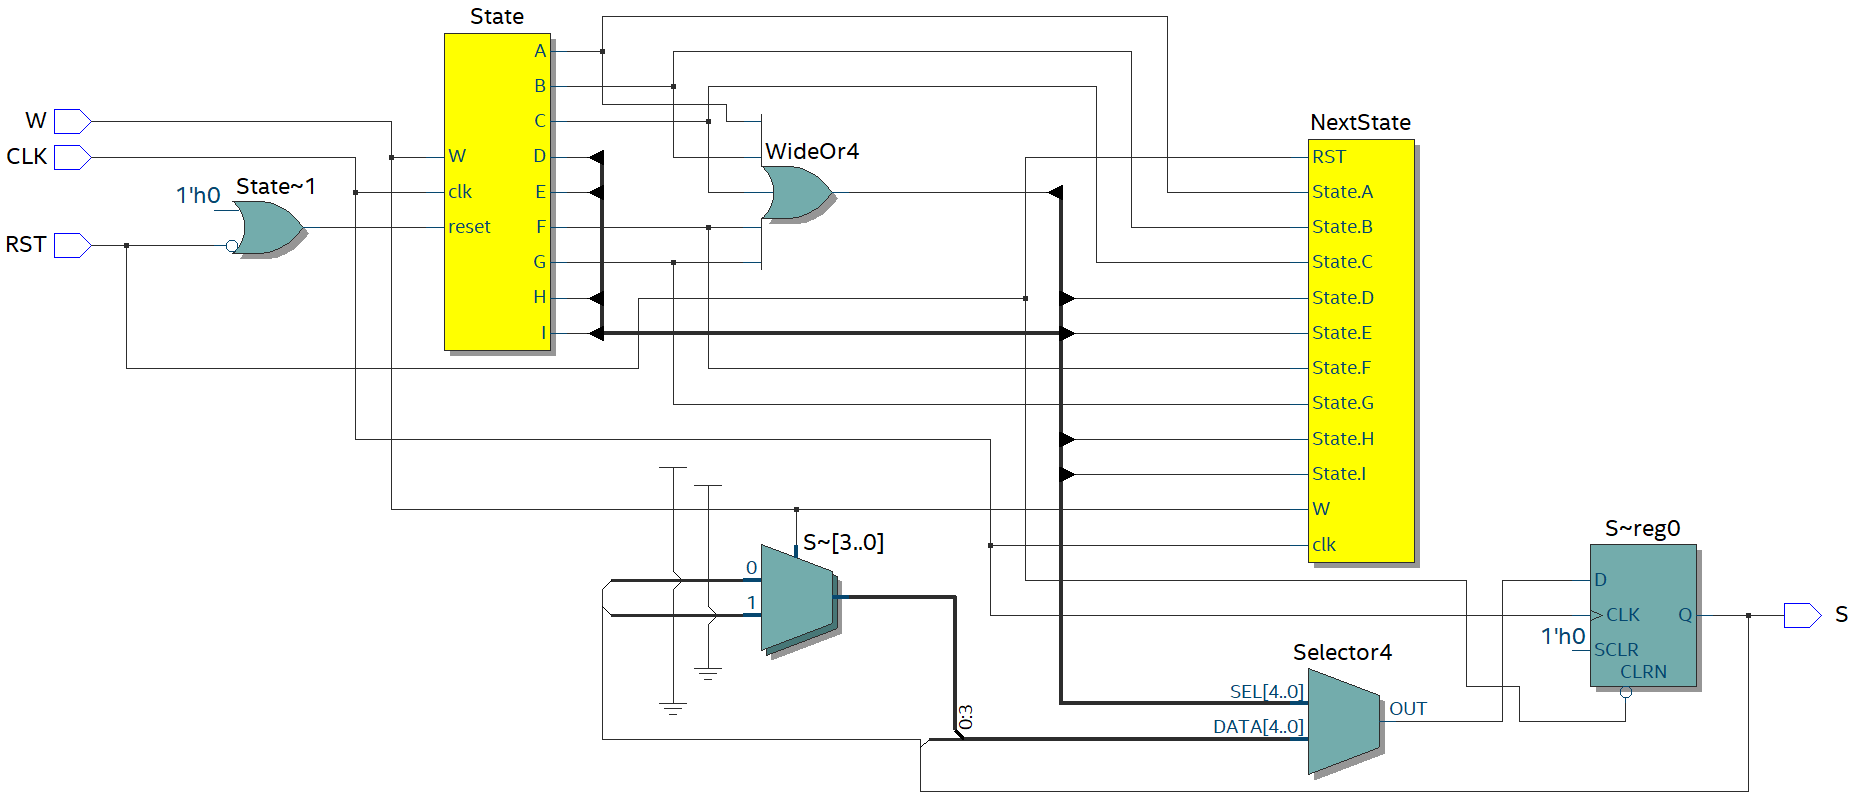
\includegraphics[scale=0.34]{FSM_Behavior_OneHot_RTL.png}
	\caption{Diagrama RTL de la FSM, descrita por comportamiento en codificación \textit{One-Hot}. \label{fig:FSM_Behavior_OneHot_RTL}}
\end{figure}

\begin{figure}[ht]
	\centering
	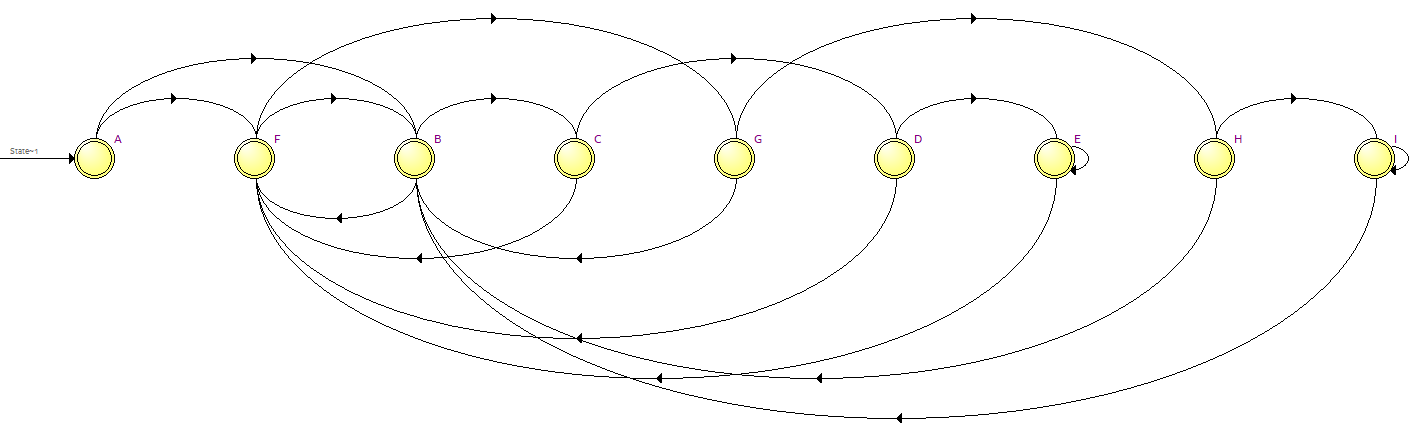
\includegraphics[scale=0.45]{FSM_Behavior_OneHot_Graph.png}
	\caption{Diagrama de estados generado por el \textit{State Machine Viewer} de la FSM estilo \textit{One-Hot}. \label{fig:FSM_Behavior_OneHot_Graph}}
\end{figure}

\begin{figure}[ht]
	\centering
	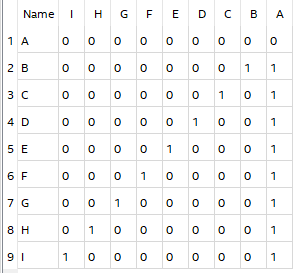
\includegraphics[scale=0.8]{FSM_Behavior_OneHot_Table.png}
	\caption{Tabla de códigos (tipo \textit{One-Hot} modificado) generada por el \textit{State Machine Viewer} de la FSM estilo \textit{One-Hot}. \label{fig:FSM_Behavior_OneHot_Table}}
\end{figure}

\begin{figure}[ht]
	\centering
	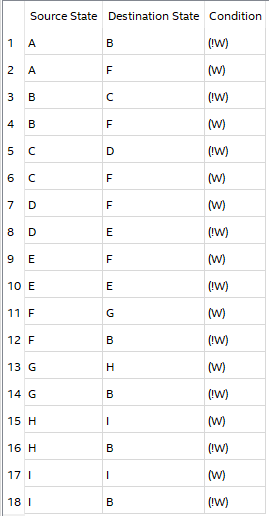
\includegraphics[scale=1.2]{FSM_Behavior_OneHot_Tran.png}
	\caption{Tabla de transiciones generada por el \textit{State Machine Viewer} de la FSM estilo \textit{One-Hot}. \label{fig:FSM_Behavior_OneHot_Tran}}
\end{figure}

\begin{figure}[ht]
	\centering
	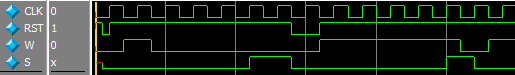
\includegraphics[scale=1.2]{FSM_OneHot_Wave.png}
	\caption{Simulación de la FSM estilo \textit{One-Hot}, en el visor de formas de onda de ModelSim. \label{fig:FSM_Behavior_OneHot_Wave}}
\end{figure}